\subsection{Operation history and machine layout}

%% ================================= history ==============================
\textbf{Operation history}

The LHC \cite{Bruning:2004ej, Buning:2004wk, Benedikt:2004wm, Evans_2008} 
is a two-ring-superconducting-hadron accelerator and collider lies in a tunnel 27 kilometres in circumference and as deep as 175 metres underground.
It's designed to provide proton-proton (pp) collisions at the centre-of-mass energy ($\sqrt{s}$) up to 14~\tev
with a unprecedented luminosity of $10^{34} cm^{-2} s^{-1}$.
In the meantime, it can also collide heavy (Pb) ions with an energy of 2.8~\tev~ per nucleon and a peak luminosity of $10^{27} cm^{-2} s^{-1}$.
Table~\ref{tab:LHC_parameters} shows the main design parameters of the LHC for proton-proton collisions.
\begin{table}[htbp]
  \centering
  \caption{Summary of design parameters of the LHC for pp collisions.}
  \label{tab:LHC_parameters}
  \begin{tabular}{cc}
    \hline
    Circumference	& 26.7 km\\
    Beam energy at collision	& 7 ~\tev\\
    Beam energy at injection	& 0.45~\tev \\
    Dipole field at 7~\tev	& 8.33 T \\
    Luminosity		& $10^{34} cm^{-2} s^{-1}$ \\
    Beam current	& 0.56 A \\
    Protons per bunch	& $1.1 \times 10^{11}$ \\
    Number of bunches	& 2808 \\
    Nominal bunch spacing	& 24.95 ns \\
    Normalized emittance	& 3.75 $\mu$m \\
    Total crossing angle	& 300 $\mu$rad \\
    Energy loss per turn	& 6.7 keV \\
    Critical synchrotron energy	& 44.1 eV \\
    Radiated power per beam	& 3.8 kW \\
    Stored energy per beam	& 350 MJ \\
    Stored energy in magnets	& 11 GJ \\
    Operating temperature	& 1.9 K \\
    \hline
  \end{tabular}
\end{table}

The LHC was built from 1998 to 2008. 
It started its first beam in September 2008, but then was interrupted by a quench incident only after a few days running.
Then it resumed the operation in November 2009 with a low energy beams.
From March 2010, physics runs took place at the centre-of-mass energy of 7~\tev.
Later on, this energy was increased in 2012 to $\sqrt{s} = 8~\tev$, with an integrated luminosity of 20.3~\ifb, and this period is called "run-1".
After run-1, the LHC was shut down for two years for hardware maintenance and upgrade, starting from February 2013.

The second operation period with higher centre-of-mass energy at 13~\tev~ started from 2015 called "run-2".
And it continued to the end of 2018 with total integrated luminosity reaching about 147 $fb^{-1}$ for ATLAS.
Figure~\ref{fig:lumi_vs_month} shows the cumulative luminosity as a function of time in month delivered to ATLAS experiment during stable beams 
in years from 2011 to 2018.
\begin{figure}[!htb]
  \centering
  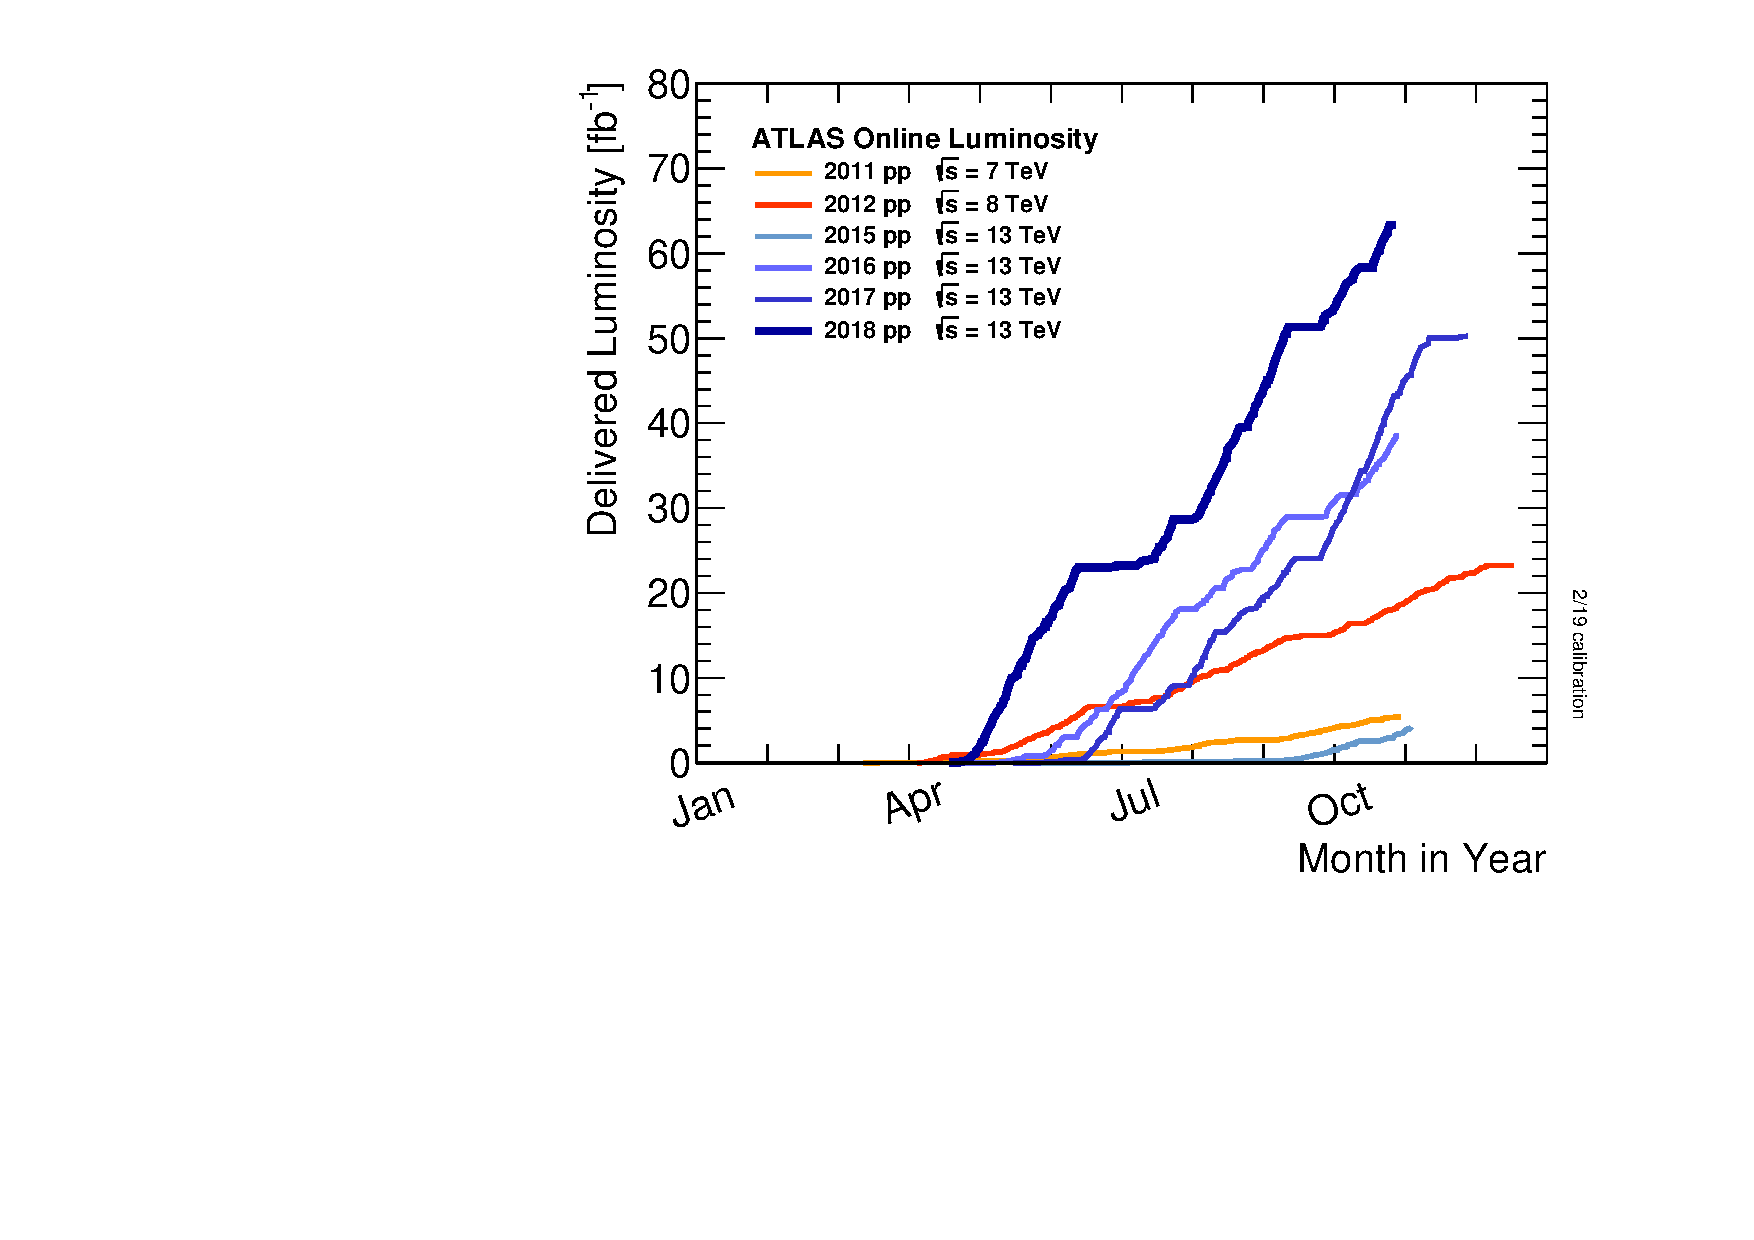
\includegraphics[width=0.6\textwidth]{figures/Detector/intlumivsyear.pdf}
  \caption{Cumulative luminosity as a function of time in years from 2011 to 2018 for ATLAS detector.}
  \label{fig:lumi_vs_month}
\end{figure}

%% ======================================= layout ==============================
\textbf{Machine layout}

The layout of CERN accelerator complex is shown in figure~\ref{cern_layout}.
The protons are accelerated by a series of machines before being injected into the main cavity.
At beginning, the 50~\mev~ protons are produced in the linear particle accelerator LINAC2, 
and then further accelerated to 1.4~\gev~ in Proton Synchrotron Booster (PSB).
The protons are then injected into the Proton Synchrotron (PS) to gain the energy of 26~\gev~ and further accelerated to 450~\gev~ in Super Proton Synchrotron (SPS).
At the end, they are injected into the main ring, and can reach a maximum energy of 7~\tev.

\begin{figure}[!htb]
  \centering
  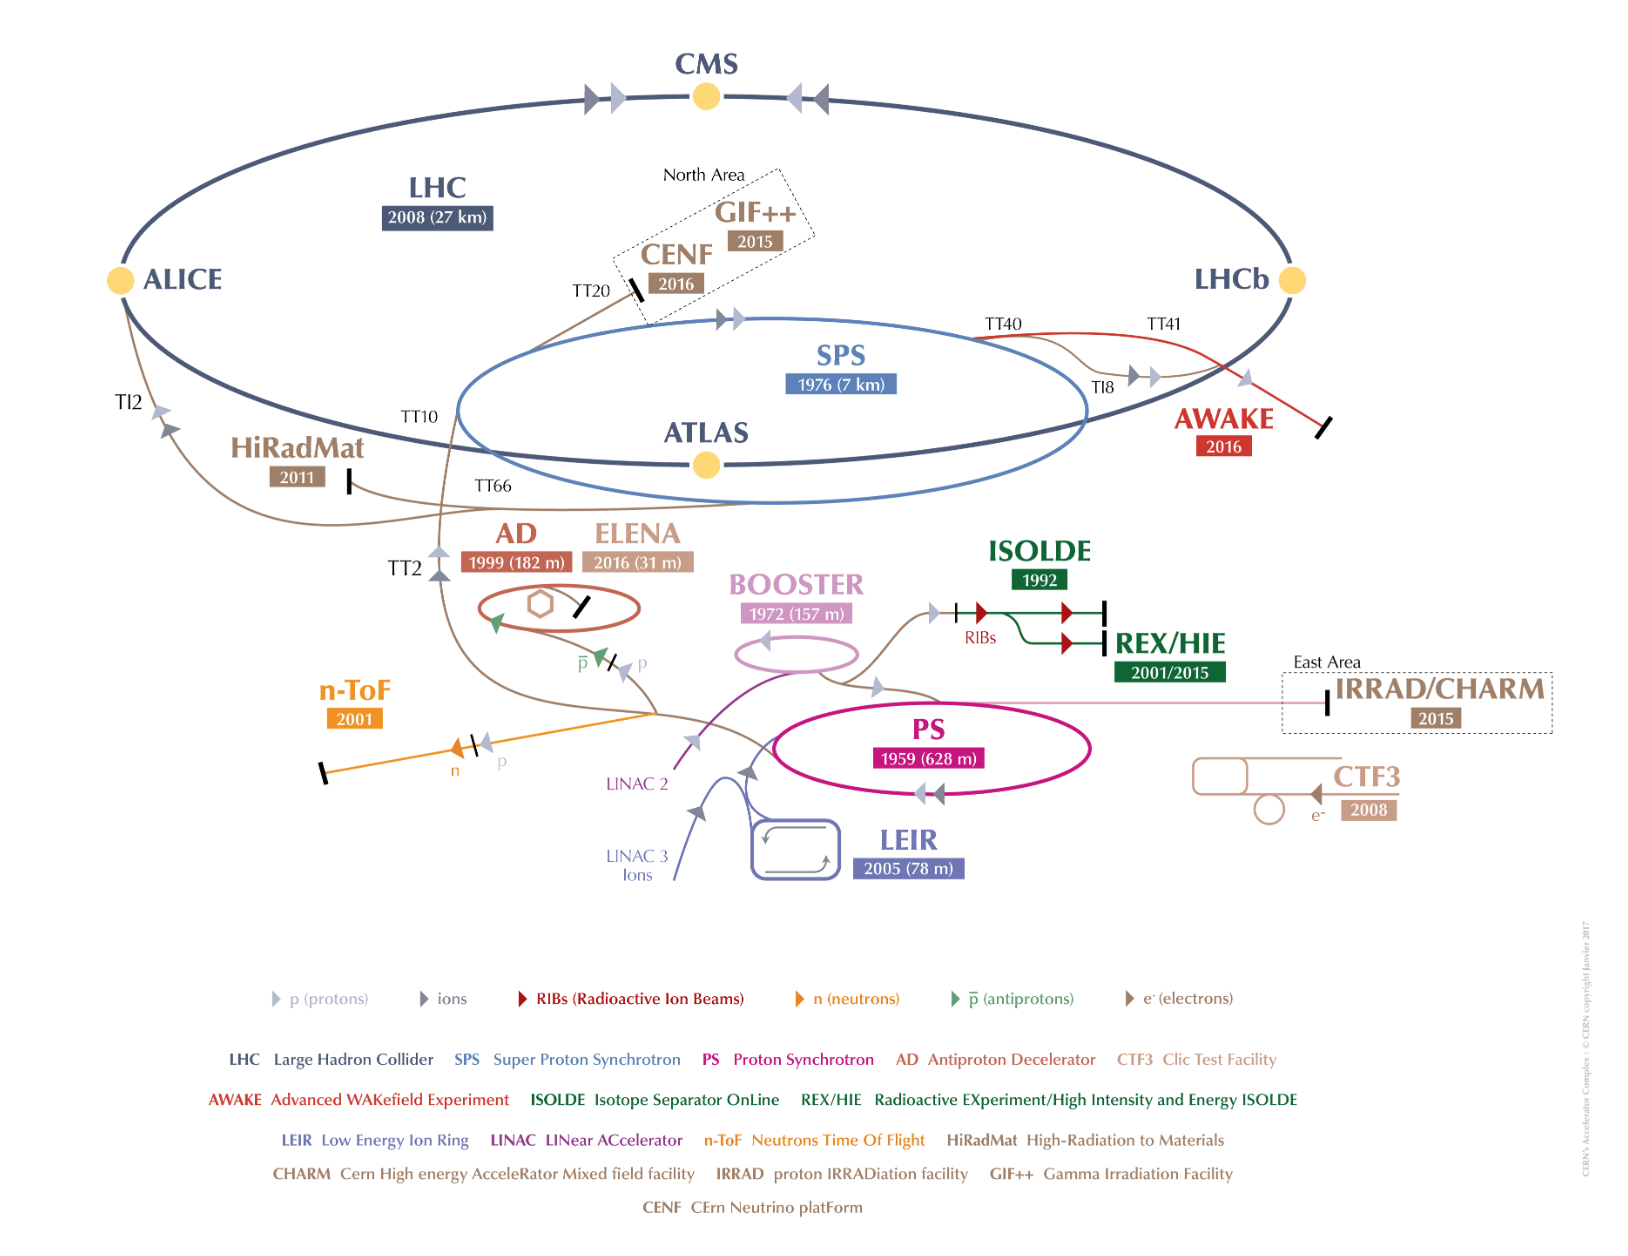
\includegraphics[width=1.0\textwidth]{figures/Detector/LHC_v2017.png}
  \caption{CERN accelerator complex \cite{Mobs:2197559}.}
  \label{cern_layout}
\end{figure}

The collisions can occur in 4 points, with corresponding 4 major detector experiments that are briefly described as follows:
\begin{itemize}
	\item \textbf{ATLAS}: A Toroidal LHC ApparatuS, one of the two general-purpose particle detector experiments and detector with largest volume at the LHC. It is designed to search for the Higgs boson, test the stardand model of particle physics and search for possible beyond SM physics.
	\item \textbf{CMS}: Compact Muon Solenoid, another large general-purpose particle physics detector, with the same physics goal (also cross check) as ATLAS.
	\item \textbf{ALICE}: A Large Ion Collider Experiment, it is optimized to study heavy-ion (Pb-Pb nuclei) collisions at a centre-of-mass energy of 2.76~\tev~ per nucleon pair.
	\item \textbf{LHCb}: Large Hadron Collider beauty, it is a specialized b-physics experiment, designed primarily to measure the parameters of CP violation in the interactions of b-hadrons.
\end{itemize}


